% =====================================================================
%  Monster Tamers — Final Project Report (DOC-2)
%  Advanced Software Engineering (Lab) — University of Pisa, A.Y. 2026/27
%  Compile: /opt/homebrew/bin/tectonic -X compile Monster_Tamers_Final_Report.tex
% =====================================================================
\documentclass[10.5pt,a4paper]{article}

% ---------------------------------------------------------------------
%  Packages
% ---------------------------------------------------------------------
\usepackage{fontspec}
\usepackage[english]{babel}
\usepackage[a4paper,top=2.3cm,bottom=2.3cm,left=2.2cm,right=2.2cm,headheight=14pt]{geometry}
\usepackage{microtype}
\usepackage{amsmath}
\usepackage{float}
\usepackage{xcolor}
\usepackage{array,booktabs,tabularx,xltabular,multirow}
\usepackage{enumitem}
\usepackage{titlesec}
\usepackage{fancyhdr}
\usepackage[font=small,labelfont=bf,labelsep=period]{caption}
\usepackage{adjustbox}
\usepackage{needspace}
\usepackage{tikz}
\usetikzlibrary{arrows.meta,positioning,shapes.geometric,fit,calc,backgrounds}
\usepackage{url}
\usepackage[hidelinks]{hyperref}

% ---------------------------------------------------------------------
%  Typography (matching architettura_backend.tex)
% ---------------------------------------------------------------------
\setmainfont{texgyrepagella}[
  Extension      = .otf,
  UprightFont    = *-regular,
  BoldFont       = *-bold,
  ItalicFont     = *-italic,
  BoldItalicFont = *-bolditalic]
\setsansfont{texgyreheros}[
  Extension      = .otf,
  UprightFont    = *-regular,
  BoldFont       = *-bold,
  ItalicFont     = *-italic,
  BoldItalicFont = *-bolditalic]
\setmonofont{lmmono10-regular}[Extension=.otf, Scale=MatchLowercase]
\usepackage{unicode-math}
\setmathfont{texgyrepagella-math.otf}

% ---------------------------------------------------------------------
%  Colors & Layout
% ---------------------------------------------------------------------
\definecolor{accent}{HTML}{1B4965}
\definecolor{accentlight}{HTML}{EEF4F8}
\definecolor{rulegray}{gray}{0.45}
\definecolor{okgreen}{HTML}{1B7A43}
\definecolor{warnamber}{HTML}{A15C00}
\definecolor{softborder}{HTML}{C9D6DF}

\titleformat{\section}{\sffamily\Large\bfseries\color{accent}}{\thesection}{0.75em}{}[\vspace{2pt}\color{softborder}\titlerule]
\titleformat{\subsection}{\sffamily\large\bfseries\color{accent}}{\thesubsection}{0.7em}{}
\titleformat{\subsubsection}{\sffamily\normalsize\bfseries}{\thesubsubsection}{0.6em}{}
\titlespacing*{\section}{0pt}{2.4ex plus 1ex minus .2ex}{1.2ex plus .2ex}
\titlespacing*{\subsection}{0pt}{1.7ex plus .8ex minus .2ex}{0.7ex plus .2ex}
\titlespacing*{\subsubsection}{0pt}{1.2ex plus .5ex minus .2ex}{0.4ex plus .1ex}

\pagestyle{fancy}
\fancyhf{}
\fancyhead[L]{\small\sffamily\color{rulegray} Monster Tamers — Final Project Report}
\fancyhead[R]{\small\sffamily\color{rulegray} Group Fantastic 4 · ASE Lab 2026/27}
\fancyfoot[C]{\small\sffamily\thepage}
\renewcommand{\headrulewidth}{0.4pt}
\renewcommand{\headrule}{\hbox to\headwidth{\color{softborder}\leaders\hrule height \headrulewidth\hfill}}

\setlength{\parindent}{0pt}
\setlength{\emergencystretch}{3em}
\setlength{\parskip}{0.48em}
\setlist{itemsep=0.15em, topsep=0.25em, leftmargin=1.5em}
\renewcommand{\arraystretch}{1.22}

\newcolumntype{L}[1]{>{\raggedright\arraybackslash}p{#1}}
\newcolumntype{R}[1]{>{\raggedleft\arraybackslash}p{#1}}
\newcolumntype{C}[1]{>{\centering\arraybackslash}p{#1}}
\newcolumntype{Y}{>{\raggedright\arraybackslash}X}

% Inline code / endpoint helpers
\DeclareRobustCommand{\code}[1]{\begingroup\def\_{\textunderscore\allowbreak}\texttt{#1}\endgroup}
\newcommand{\codec}[1]{\texttt{\detokenize{#1}}}
\DeclareUrlCommand\ep{\urlstyle{tt}\def\UrlBreaks{\do\/}}

% Status badges
\newcommand{\badgeok}[1]{\textsf{\textbf{\color{okgreen}#1}}}
\newcommand{\badgewarn}[1]{\textsf{\textbf{\color{warnamber}#1}}}
\newcommand{\badgeinfo}[1]{\textsf{\textbf{\color{accent}#1}}}

% Callout box
\newenvironment{callout}[1]{%
  \par\medskip\noindent
  \begin{tabular}{|p{\dimexpr\linewidth-2\tabcolsep-2\arrayrulewidth\relax}|}
  \hline
  \rowcolor{accentlight}\sffamily\bfseries\small\color{accent} #1 \\
  \hline
  \vspace{0.15em}\small
}{%
  \vspace{0.15em}\\
  \hline
  \end{tabular}\par\medskip
}
\usepackage{colortbl}

% ---------------------------------------------------------------------
%  TikZ Styles (Architecture & Sequence Diagrams)
% ---------------------------------------------------------------------
\tikzset{
  arr/.style={-{Stealth[length=2.0mm]}, thick, color=accent},
  darr/.style={-{Stealth[length=2.0mm]}, thick, densely dashed, color=rulegray},
  comp/.style={draw=accent, thick, rounded corners=3pt, minimum width=2.1cm, minimum height=0.72cm,
               font=\sffamily\footnotesize\bfseries, align=center, fill=white, text depth=0.2ex},
  gw/.style={draw=accent, very thick, rounded corners=3pt, minimum width=2.4cm, minimum height=1.1cm,
             font=\sffamily\footnotesize\bfseries, align=center, fill=accentlight, text depth=0.2ex},
  db/.style={draw=rulegray, thick, cylinder, shape border rotate=90, aspect=0.22,
             minimum width=1.45cm, minimum height=0.72cm, fill=white,
             font=\sffamily\scriptsize, align=center},
  tbbox/.style={draw=softborder, thick, dashed, rounded corners=5pt, inner sep=7pt},
}

\newcommand{\lifeline}[3]{%
  \node[draw=accent, fill=accentlight, rounded corners=2pt, minimum width=1.95cm, minimum height=0.58cm,
        font=\sffamily\scriptsize\bfseries, align=center] at (#1,0) {#2};
  \draw[rulegray, densely dashed] (#1,-0.30) -- (#1,#3);}
\newcommand{\smsg}[4]{%
  \draw[arr] (#1,#3) -- node[above, font=\ttfamily\scriptsize, align=center, inner sep=1.2pt, fill=white]{#4} (#2,#3);}
\newcommand{\srmsg}[4]{%
  \draw[darr] (#1,#3) -- node[above, font=\sffamily\scriptsize, align=center, inner sep=1.2pt, fill=white]{#4} (#2,#3);}
\newcommand{\sself}[3]{%
  \draw[arr] (#1,#2) -- ++(0.35,0) -- ++(0,-0.28) -- ++(-0.35,0);
  \node[anchor=west, font=\sffamily\scriptsize, align=left] at ($(#1,#2)+(0.40,-0.14)$) {#3};}
\newcommand{\sfrag}[6]{%
  \draw[rulegray] (#1,#2) rectangle (#3,#4);
  \node[draw=rulegray, fill=accentlight, anchor=north west, font=\sffamily\scriptsize\bfseries, inner sep=2pt] at (#1,#2) {#5};
  \node[anchor=north west, font=\sffamily\scriptsize] at ($(#1,#2)+(0.85,-0.02)$) {[#6]};}
\newcommand{\sfragsep}[4]{%
  \draw[rulegray, dashed] (#1,#3) -- (#2,#3);
  \node[anchor=north west, font=\sffamily\scriptsize] at (#1,#3) {[#4]};}

% ---------------------------------------------------------------------
%  PDF Metadata
% ---------------------------------------------------------------------
\hypersetup{
  pdftitle={Monster Tamers — Final Project Report},
  pdfauthor={Group Fantastic 4: Giacomo Cesaretti, Federico Lombardi, Fabio Piscitelli, Francesco Polperio},
  pdfsubject={Advanced Software Engineering (Lab), University of Pisa, A.Y. 2026/27},
}

% =====================================================================
\begin{document}
% =====================================================================

% ---------------------------------------------------------------------
%  Title Page
% ---------------------------------------------------------------------
\hypersetup{pageanchor=false}
\begin{titlepage}
  \sffamily
  \vspace*{0.6cm}
  {\large\bfseries\color{accent} University of Pisa}\\[0.25em]
  {\normalsize Department of Computer Science \quad·\quad Advanced Software Engineering (Lab) \quad·\quad A.Y. 2026/27}

  \vspace{0.5cm}
  {\color{accent}\rule{\linewidth}{1.2pt}}

  \vspace{2.4cm}
  {\fontsize{34}{40}\selectfont\bfseries\color{accent} Monster Tamers}\\[0.6em]
  {\LARGE\bfseries Final Project Report}\\[0.45em]
  {\large Architecture, Engineering Rationale, Security Assessment, and Verification}

  \vspace{1.6cm}
  \begin{tabularx}{\linewidth}{@{}L{3.6cm}Y@{}}
    \toprule
    \textbf{Group}        & \textbf{Fantastic 4} \\
    \textbf{Team Members} & Giacomo Cesaretti (\code{giacomocesaretti03@gmail.com}) \\
                          & Federico Lombardi (\code{f.lombardi26@studenti.unipi.it}) \\
                          & Fabio Piscitelli (\code{f.piscitelli4@studenti.unipi.it}) \\
                          & Francesco Polperio (\code{f.polperio@studenti.unipi.it}) \\
    \midrule
    \textbf{Instructor}   & Alessandro Bocci \\
    \textbf{Delivery}     & Final Release (\code{v1.0-final}, Phase 2) — Due 15 December 2026 \\
    \textbf{Verified On}  & 27 November 2026 (branch \code{main}) \\
    \textbf{Repository}   & \url{https://github.com/fabiopsh/ASE-Tamer-Project} \\
    \bottomrule
  \end{tabularx}

  \vfill
  \begin{callout}{Executive Verification Snapshot (27 November 2026)}
    \textbf{Architecture:} 6 Quarkus 3.39.5 / Java 21 microservices, Nginx HTTPS API gateway, 6 isolated PostgreSQL 17 databases on dedicated internal networks, separate React 19 / TypeScript / Vite 8 frontend stack.\\
    \textbf{Functional Scope:} 25 of 28 backlog stories implemented — all 18 mandatory red, both yellow (\code{US-05}, \code{US-25}), and 5 optional green stories (\code{US-04}, \code{US-07}, \code{US-13}, \code{US-21}, \code{US-22}).\\
    \textbf{Automated Verification:} \textbf{273/273} JUnit/\code{@QuarkusTest} · \textbf{16/16} Vitest (0 lint/type errors, 0 prod vulns) · \textbf{399/399} Bruno API tests · \textbf{47/47} \code{SEC-1} self-attack checks · \textbf{18/18} audit-log assertions · Locust P2 \textbf{3,334 reqs / 0.00\% failures} (\code{p50} 20 ms, \code{p95} 230 ms) · Full browser playtest won through Stage 8 Boss \emph{Omnivoid} (Turn 23, 30 verified hash-chained history records).
  \end{callout}
  \vspace{0.3cm}
\end{titlepage}
\hypersetup{pageanchor=true}

% ---------------------------------------------------------------------
%  Table of Contents
% ---------------------------------------------------------------------
\setcounter{tocdepth}{2}
\tableofcontents
\clearpage

% =====================================================================
\section{Executive Summary \& Game Rules}
\label{sec:exec-summary}
% =====================================================================

\emph{Monster Tamers} is a headless, microservice-based roguelike monster-taming game built for the Advanced Software Engineering Laboratory at the University of Pisa. The system implements the required core loop—\emph{Prepare} $\rightarrow$ \emph{Encounter} $\rightarrow$ \emph{Outcome} $\rightarrow$ \emph{Progress}—with strict separation between a server-authoritative distributed backend (six Quarkus/Java 21 microservices behind an Nginx HTTPS API gateway) and a minimal, decoupled React/TypeScript web frontend deployed in its own Docker Compose stack.

Both Phase 1 (prototype) and Phase 2 (final delivery) are complete. Every mandatory functional requirement, security control from §6 of the specification, Access Security alignment (17/11/2026), and Security Assessment deliverable (18/11/2026) has been implemented and verified end to end.

\subsection{Core Loop and Roguelike Run Lifecycle}

Players progress through discrete \textbf{roguelike runs} (decision \textbf{R1}):
\begin{enumerate}
  \item \textbf{Account \& Profile:} A player registers (\ep{POST /api/auth/register}), logs in (\ep{POST /api/auth/token}), and may optionally customize display name and avatar (\ep{PATCH /api/players/me}, \code{US-04}).
  \item \textbf{Starter Selection:} Each new run generates a persistent pool of 10 distinct \code{common} species. The player chooses exactly 3 starters (\ep{POST /api/players/me/starters}, \code{US-06}/\code{US-07}), which opens the run at Stage~1.
  \item \textbf{Prepare:} Players inspect the 100-species catalogue, manage their personal collection (including custom nicknames, \code{US-13}), and assemble up to 5 validated teams of 1–3 active monsters from the current run (\code{US-14}–\code{US-16}). Duplicate species are allowed; repeating the same instance ID is rejected.
  \item \textbf{Encounter:} Each of the \textbf{8 stages} provides 3 replayable normal encounter templates and 1 stage boss (\textbf{R2}, \textbf{R12}, \textbf{R13}). Previously cleared normal templates remain playable for XP farming. After \textbf{2 wins} in the current stage, that stage's boss unlocks and can be defeated once per run.
  \item \textbf{Turn-Based Relay Battle:} Battles are interactive 1v1 relays (\textbf{R3}–\textbf{R5}): the team fights one monster at a time in slot order while the wild monster retains damage across switches. Every round the client sends a single intent—\code{attack}, \code{switch} (to a living bench slot), or \code{flee}—never outcomes or HP values.
  \item \textbf{Outcome \& Progression:}
    \begin{itemize}
      \item \textbf{Victory:} The wild monster joins the player's collection \emph{at its wild level} (\textbf{R6}, so late-stage captures are immediately usable), and every team member—including benched members—receives XP (\textbf{R11}). Beating a stage boss advances the stage; beating Stage~8 Boss \textbf{Omnivoid} marks the run \code{won} (\textbf{R16}).
      \item \textbf{Defeat / Abandon:} If the entire team is knocked out or the player abandons the run (\textbf{R14}, \textbf{R17}), the run ends (\code{lost}/\code{abandoned}) and triggers a complete orchestrated reset: active monsters are \textbf{archived} (never deleted, preserving inspectability of past runs, \textbf{R15}), teams are cleared, and a new run with a fresh 10-monster starter pool is created.
      \item \textbf{Flee / Expiry / Interruption:} A successful flee (\code{fled}), 30-minute idle timeout (\code{expired}), or service restart (\code{interrupted}) closes the battle with no reward while keeping the run alive.
    \end{itemize}
\end{enumerate}

\subsection{Catalogue, Stages, and Boss Balance}

The static catalogue seeded in \code{monsters} contains \textbf{100 monster species} across \textbf{7 elements} (\code{dream}, \code{echo}, \code{silence}, \code{memory}, \code{time}, \code{gravity}, \code{chaos}), \textbf{3 rarities} (\code{common}, \code{rare}, \code{legendary}), and \textbf{28 distinct abilities}, each with custom pixel-art sprites served publicly from \ep{/images/monsters/{NNN}.png}. The 8 stage bosses are excluded from wild rolls (\textbf{P-21}) so each boss is obtainable exclusively by defeating it.

\begin{table}[H]
\centering
\caption{Eight-stage roguelike progression and boss ladder (\code{encounter\_templates}, 32 templates total).}
\label{tab:stages}
\footnotesize
\begin{tabularx}{\linewidth}{@{}C{0.9cm}C{1.4cm}L{3.5cm}C{2.4cm}L{4.8cm}C{1.3cm}@{}}
\toprule
\textbf{Stage} & \textbf{Wild Lvl} & \textbf{Normal Elements} & \textbf{Weights (C/R/L)} & \textbf{Stage Boss (ID, Element, Rarity)} & \textbf{Boss Lvl} \\
\midrule
1 & 1–3   & dream, echo, silence   & 100 / 0 / 0   & Loomwidow (31, memory, rare)        & 5  \\
2 & 4–6   & memory, time, gravity  & 90 / 10 / 0   & Frostveil (89, silence, rare)       & 8  \\
3 & 7–9   & dream, echo, silence   & 80 / 20 / 0   & Nebulynx (74, gravity, rare)        & 11 \\
4 & 10–12 & memory, time, gravity  & 70 / 30 / 0   & Choraleth (62, echo, legendary)     & 14 \\
5 & 13–15 & dream, silence, chaos  & 60 / 40 / 0   & Chronarch (47, time, legendary)     & 17 \\
6 & 16–18 & echo, memory, gravity  & 50 / 45 / 5   & Morpheon (16, dream, legendary)     & 20 \\
7 & 19–21 & time, silence, chaos   & 40 / 50 / 10  & Quietus (92, silence, legendary)    & 23 \\
8 & 22–24 & dream, gravity, chaos  & 30 / 55 / 15  & \textbf{Omnivoid} (100, chaos, legendary) & 26 \\
\bottomrule
\end{tabularx}
\end{table}

\subsection{Deterministic Battle Engine v2, Formulas, and Abilities}

The battle engine (\code{it.unipi.ase.tamer.encounters.engine}) is pure Java with zero framework or database dependencies, making it trivially unit-testable and deterministic. Every battle is initialized with a 64-bit seed from \code{SecureRandom} driving a dedicated \code{java.util.SplittableRandom(seed)}. The exact order of random draws—wild rarity $\rightarrow$ species $\rightarrow$ level $\rightarrow$ per-round speed tie-break $\rightarrow$ per-attack dodge roll (if active) $\rightarrow$ damage variance—is versioned by \code{Battle.ENGINE\_VERSION = 2} and persisted with \code{rng\_seed} in \code{history} for verifiable replays.

\textbf{Core Formulas:}
\begin{align*}
\text{stat}_{\text{eff}} &= \text{base} + \text{growth} \times (\text{level} - 1) \qquad (\text{computed solely in \texttt{monsters}; max level 50}) \\
\text{HP}_{\max}(\text{team}) &= 2 \cdot \text{hp}_{\text{eff}} + 10, \qquad
\text{HP}_{\max}(\text{wild}) = \text{round}\big(\text{HP}_{\max}(\text{team}) \times m\big), \quad m = \begin{cases} 1.50 & \text{wild} \\ \mathbf{1.25} & \text{boss} \end{cases} \\
\text{damage} &= \max\!\left(1,\; \text{round}\!\left(\frac{\text{atk}^2}{\text{atk} + \text{def}} \times 0.6 \times \text{elem} \times \text{var} \times \text{boost} \times \text{reduction}\right)\right) \\
p_{\text{flee}} &= \min\!\left(0.95,\; \frac{\text{speed}_{\text{active}}}{\text{speed}_{\text{active}} + \text{speed}_{\text{wild}}} + 0.25\right) \\
\text{XP}_{\text{win}} &= \text{round}\big(10 \cdot \text{lvl}_{\text{wild}} \cdot w_{\text{rarity}}\big), \qquad \text{XP}_{\text{next}} = 15 \cdot \text{lvl}
\end{align*}
where $\text{elem} \in \{1.5, 0.67, 1.0\}$, $\text{var} \sim U[0.9, 1.1]$, and $w_{\text{rarity}} \in \{1.0, 1.5, 2.0\}$ for common/rare/legendary.

\textbf{Boss Balance Tuning (\code{EN-6}):} The original architecture proposed a $2.5\times$ boss HP multiplier, under which \code{BalanceSimulation} (1,000 battles/template) showed 0–15\% win rates from Stage~3 onward because bosses already enjoy a $+2$ level advantage and higher rarity growth. Phase~1 lowered the multiplier to $1.5\times$, and Phase~2—once all 7 complex abilities (such as boss \code{heal}, \code{reflect}, \code{stun}, and \code{invert\_advantage}) became active—further tuned \code{HpCalculator.BOSS\_HP\_MULTIPLIER = 1.25}, keeping bosses challenging while making Stage~8 \emph{Omnivoid} beatable in a full interactive playthrough.

\textbf{All 28 Abilities (P1 + P2):} Ability effects are declarative data (\code{effect\_type}, \code{effect\_value}, \code{trigger}) evaluated exclusively on the server across triggers \code{always}, \code{first\_turn}, \code{hp\_below\_50}, \code{hp\_above\_50}, \code{vs\_faster}, \code{on\_hit}, \code{on\_attack}, and \code{once}.

\begin{table}[H]
\centering
\caption{Complete ability effect matrix in Battle Engine v2 (\code{AbilityEngine}).}
\label{tab:abilities}
\footnotesize
\begin{tabularx}{\linewidth}{@{}L{3.1cm}C{1.1cm}Y L{2.4cm}@{}}
\toprule
\textbf{Effect Type} & \textbf{Phase} & \textbf{Server-Side Behaviour} & \textbf{Ability IDs} \\
\midrule
\code{damage\_boost}        & P1 & Multiplies outgoing damage by $(1 + v/100)$ & 4, 10, 15, 18, 21 \\
\code{damage\_reduction}    & P1 & Multiplies incoming damage by $(1 - v/100)$ & 1, 5, 14, 25 \\
\code{speed\_boost}         & P1 & Multiplies effective speed by $(1 + v/100)$ & 6, 13 \\
\code{dodge}               & P1 & $v\%$ chance to negate an incoming attack (0 damage) & 2, 9, 17 \\
\code{weaken}              & P1 & Scales opponent attack by $(1 - v/100)$ while active & 16, 26 \\
\code{ignore\_disadvantage} & P1 & Converts disadvantageous \code{elem} $0.67 \rightarrow 1.0$ when attacking & 19 \\
\midrule
\code{heal}                & P2 & First time HP falls below 50\%, restores $v\%$ of max HP (\code{ability} event) & 3, 12 \\
\code{reflect}             & P2 & Deals $\max(1, \lfloor v\% \times \text{damage taken}\rfloor)$ back to attacker & 7, 11, 23 \\
\code{stun}                & P2 & After dealing damage, $v\%$ chance target skips its next action & 8, 22 \\
\code{revive}              & P2 & Once per encounter on KO, revives with $v\%$ max HP & 24 \\
\code{random\_boost}        & P2 & Each action, boosts one randomly chosen stat (atk/def/spd) by $v\%$ & 20 \\
\code{copy\_ability}        & P2 & On first round, copies opponent's ability for the rest of the battle & 27 \\
\code{invert\_advantage}    & P2 & While on field, swaps \code{elem} $1.5 \leftrightarrow 0.67$ for both sides & 28 \\
\bottomrule
\end{tabularx}
\end{table}

% =====================================================================
\section{Architecture \& Design Rationale}
\label{sec:architecture}
% =====================================================================

\subsection{High-Level Component and Network Topology}

The backend is a \textbf{headless} Docker Compose stack (\code{docker-compose.yml}) exposing a single published port (\code{127.0.0.1:8443}) on the Nginx API gateway. The React frontend runs in a completely separate Compose stack (\code{docker-compose.frontend.yml}, \code{127.0.0.1:8080}) and communicates exclusively with the gateway over HTTPS with CORS.

Inside the backend stack, services communicate over an \code{internal: true} bridge network (\code{backend}). Each of the six PostgreSQL 17 databases resides on its own dedicated internal network (\code{<svc>-db-net}), ensuring neither the gateway nor any foreign microservice has a network route to another service's database. A one-shot, networkless (\code{network\_mode: none}) \code{init-secrets} container bootstraps the local CA, per-container TLS certificates, RSA JWT key pair, DB passwords, service client secrets, and AES/HMAC keys into a named Docker volume mounted read-only per subpath.

\begin{figure}[H]
\centering
\begin{adjustbox}{max width=\linewidth}
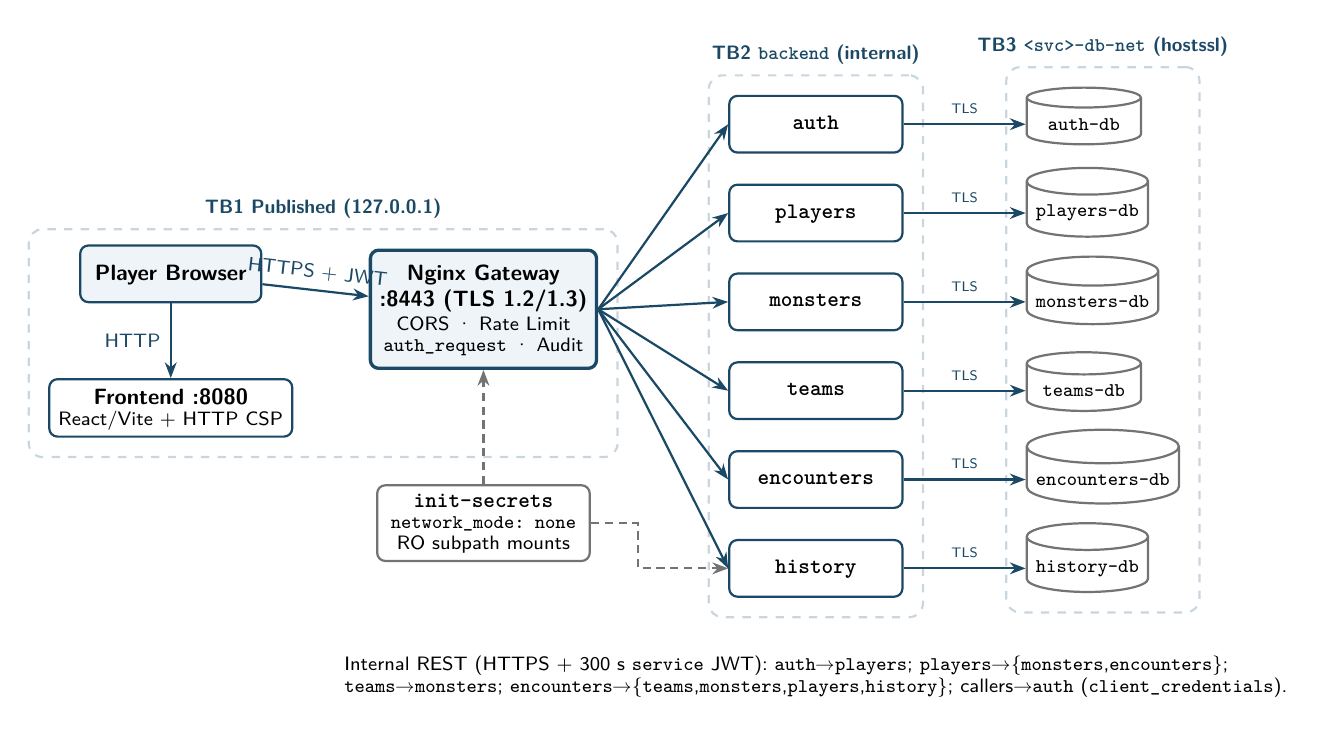
\begin{tikzpicture}[node distance=0.8cm and 0.9cm]
  % External actors
  \node[comp, fill=accentlight, minimum width=2.3cm] (browser) {Player Browser};
  \node[comp, below=0.95cm of browser, minimum width=2.3cm] (fe) {Frontend :8080\\[-2pt]\scriptsize\mdseries React/Vite + HTTP CSP};

  % Gateway
  \node[gw, right=1.35cm of browser, yshift=-0.45cm, minimum width=2.7cm, minimum height=1.5cm] (gw) {Nginx Gateway\\:8443 (TLS 1.2/1.3)\\[-1pt]\scriptsize\mdseries CORS · Rate Limit\\[-2pt]\scriptsize\mdseries \code{auth\_request} · Audit};

  % 6 Services
  \node[comp, right=1.65cm of gw, yshift=2.35cm, minimum width=2.2cm] (auth) {\code{auth}};
  \node[comp, below=0.38cm of auth, minimum width=2.2cm] (players) {\code{players}};
  \node[comp, below=0.38cm of players, minimum width=2.2cm] (monsters) {\code{monsters}};
  \node[comp, below=0.38cm of monsters, minimum width=2.2cm] (teams) {\code{teams}};
  \node[comp, below=0.38cm of teams, minimum width=2.2cm] (enc) {\code{encounters}};
  \node[comp, below=0.38cm of enc, minimum width=2.2cm] (hist) {\code{history}};

  % 6 DBs
  \node[db, right=1.55cm of auth] (dba) {\code{auth-db}};
  \node[db, right=1.55cm of players] (dbp) {\code{players-db}};
  \node[db, right=1.55cm of monsters] (dbm) {\code{monsters-db}};
  \node[db, right=1.55cm of teams] (dbt) {\code{teams-db}};
  \node[db, right=1.55cm of enc] (dbe) {\code{encounters-db}};
  \node[db, right=1.55cm of hist] (dbh) {\code{history-db}};

  % init-secrets
  \node[comp, below=1.45cm of gw, fill=white, draw=rulegray, minimum width=2.7cm] (init) {\code{init-secrets}\\[-2pt]\scriptsize\mdseries \code{network\_mode: none}\\[-2pt]\scriptsize\mdseries RO subpath mounts};

  % Trust boundary boxes
  \begin{scope}[on background layer]
    \node[tbbox, fit=(fe)(gw), label={[font=\sffamily\scriptsize\bfseries, color=accent]above:TB1 Published (127.0.0.1)}] (tb1) {};
    \node[tbbox, fit=(auth)(players)(monsters)(teams)(enc)(hist), label={[font=\sffamily\scriptsize\bfseries, color=accent]above:TB2 \code{backend} (internal)}] (tb2) {};
    \node[tbbox, fit=(dba)(dbp)(dbm)(dbt)(dbe)(dbh), label={[font=\sffamily\scriptsize\bfseries, color=accent]above:TB3 \code{<svc>-db-net} (hostssl)}] (tb3) {};
  \end{scope}

  % Arrows
  \draw[arr] (browser) -- node[left, font=\sffamily\scriptsize]{HTTP} (fe);
  \draw[arr] (browser) -- node[above, font=\sffamily\scriptsize, sloped]{HTTPS + JWT} (gw);
  \draw[arr] (gw.east) -- (auth.west);
  \draw[arr] (gw.east) -- (players.west);
  \draw[arr] (gw.east) -- (monsters.west);
  \draw[arr] (gw.east) -- (teams.west);
  \draw[arr] (gw.east) -- (enc.west);
  \draw[arr] (gw.east) -- (hist.west);

  % DB arrows
  \foreach \s/\d in {auth/dba, players/dbp, monsters/dbm, teams/dbt, enc/dbe, hist/dbh} {
    \draw[arr] (\s.east) -- node[above, font=\sffamily\tiny]{TLS} (\d.west);
  }

  % Secrets dashed
  \draw[darr] (init.north) -- (gw.south);
  \draw[darr] (init.east) -- ++(0.6,0) |- (hist.west);

  % Service-to-service summary note
  \node[font=\sffamily\scriptsize, align=left, below=0.35cm of tb2.south, anchor=north]
    {Internal REST (HTTPS + 300 s \code{service} JWT): \code{auth}$\to$\code{players}; \code{players}$\to$\{\code{monsters},\code{encounters}\};\\
     \code{teams}$\to$\code{monsters}; \code{encounters}$\to$\{\code{teams},\code{monsters},\code{players},\code{history}\}; callers$\to$\code{auth} (\code{client\_credentials}).};
\end{tikzpicture}
\end{adjustbox}
\caption{Monster Tamers deployment topology and trust boundaries (TB1–TB3; TB4 covers CI build \& \code{init-secrets}).}
\label{fig:arch}
\end{figure}

\subsection{Per-Service Responsibilities, APIs, and Persistence}

Every service runs Quarkus 3.39.5 on Java 21 with Hibernate ORM / Panache and Flyway SQL/Java migrations (\textbf{A1}, \textbf{A8}). No shared Maven code module exists (\textbf{A9}): each service owns its DTOs, REST clients, and domain tables, sharing only the canonical \code{backend/security/access-policy.json} resource (\textbf{P-24}). Public routes require a verified \code{player} JWT (except auth endpoints and public sprites), internal routes live under \ep{/internal/*} (blocked with \code{404} at Nginx, requiring \code{service} JWT), and \code{player\_id} is always derived from the verified JWT \code{sub} claim—never from client input. Foreign-owned resources always return \code{404 NOT\_FOUND} (\textbf{P-11}).

\begin{table}[H]
\centering
\caption{Microservices catalog: bounded context, primary endpoints, database schema, and mapped user stories.}
\label{tab:services}
\footnotesize
\begin{tabularx}{\linewidth}{@{}L{1.6cm}L{3.2cm}Y L{3.1cm}L{1.55cm}@{}}
\toprule
\textbf{Service} & \textbf{Responsibilities} & \textbf{Key Public \& Internal Endpoints} & \textbf{DB Schema (Flyway)} & \textbf{Stories} \\
\midrule
\code{auth} &
Accounts, bcrypt, AES-GCM usernames, HMAC blind index, login backoff, OAuth2 grants, RS256 signing, refresh rotation, logout, gateway auth adapter, JSON audit log &
\ep{POST /api/auth/register}, \ep{/api/auth/token} (\code{password}, \code{refresh\_token}), \ep{/api/auth/logout}; \ep{POST /internal/auth/token} (\code{client\_credentials}); \ep{GET /internal/auth/authorize} &
\code{accounts} (\code{username\_enc}, \code{username\_hmac}, \code{password\_hash}, backoff cols), \code{refresh\_tokens} (\code{token\_hash}, \code{family\_id}) &
US-01, US-02, US-05 \\
\addlinespace
\code{players} &
Player profile (\code{display\_name}, \code{avatar}), persistent 10-starter pool per run, starter selection orchestration &
\ep{GET/PATCH /api/players/me}, \ep{GET/POST /api/players/me/starters}; \ep{POST /internal/players}, \ep{POST /internal/players/{pid}/new-run} &
\code{players} (\code{player\_id}, \code{display\_name}, \code{avatar}, \code{current\_run\_id}, \code{starter\_pool}, \code{starters\_chosen}) &
US-03, US-04, US-06, US-07 \\
\addlinespace
\code{monsters} &
100-species catalogue, 28 abilities, 7 elements, public PNG sprites, per-run owned collection, nicknames, stat/XP/level formulas &
\ep{GET /api/monsters}, \ep{/monsters/{id}}, \ep{/abilities}, \ep{/elements}, \ep{/collection}, \ep{PATCH /api/collection/{id}}, \ep{GET /images/monsters/{f}}; \ep{/internal/monsters}, \ep{/stats}, \ep{/collections/{pid}/} (\code{starters}, \code{monsters}, \code{xp}, \code{instances}, \code{archive}) &
\code{monsters}, \code{abilities}, \code{elements} (seeded), \code{owned\_monsters} (\code{owned\_id}, \code{run\_id}, \code{level}, \code{xp}, \code{nickname}, \code{status}, \code{encounter\_id}) &
US-09, US-10, US-11, US-12, US-13 \\
\addlinespace
\code{teams} &
Team CRUD (1–3 slots, max 5 teams/run), live validation, battle-start revalidation, run reset &
\ep{GET/POST /api/teams}, \ep{GET/PUT/DELETE /api/teams/{id}}, \ep{POST /api/teams/validate}; \ep{GET /internal/teams/{id}}, \ep{POST /internal/teams/{pid}/reset} &
\code{teams} (\code{team\_id}, \code{player\_id}, \code{run\_id}, \code{name}), \code{team\_slots} (\code{team\_id}, \code{position}, \code{owned\_id}) &
US-14, US-15, US-16 \\
\addlinespace
\code{encounters} &
32 stage templates, run lifecycle, in-memory deterministic Battle Engine v2, outbox, sweep scheduler, reset saga &
\ep{GET /api/encounters}, \ep{/runs}, \ep{/runs/current}, \ep{POST /api/runs}, \ep{/runs/current/abandon}, \ep{POST /api/battles}, \ep{GET /api/battles/current}, \ep{POST /api/battles/current/actions}; \ep{POST /internal/runs} &
\code{encounter\_templates} (32 seeded), \code{runs} (\code{stage}, \code{wins\_in\_stage}, \code{bosses\_defeated}, \code{reset\_pending}), \code{battle\_completions} (outbox) &
US-17, US-18, US-19, US-20, US-21, US-22 \\
\addlinespace
\code{history} &
Permanent append-only battle log, per-player SHA-256 hash chain, integrity verification endpoint &
\ep{GET /api/history}, \ep{/api/history/{id}}, \ep{GET /api/history/verify}; \ep{POST /internal/history} &
\code{encounter\_records} (append-only trigger, JSONB \code{turns}/\code{wild}/\code{team\_snapshot}, \code{seq}, \code{prev\_hash}, \code{hash}), \code{chain\_heads} &
US-23, US-24, US-25 \\
\bottomrule
\end{tabularx}
\end{table}

\subsection{Consolidated Design Decision Log (A1–A9, R1–R20, P-01–P-28)}

Every architectural choice made from kickoff (15/10/2026) through the implementation plan (06/11/2026), Access Security review (17/11/2026), and Security Assessment lab (18/11/2026) is tracked below.

\begin{xltabular}{\linewidth}{@{}L{1.15cm}L{3.1cm}Y@{}}
\caption{Consolidated Decision Log: Architecture (A1–A9), Game Rules (R1–R20), and Plan/Security (P-01–P-28).}\label{tab:decisions}\\
\toprule
\textbf{ID} & \textbf{Topic} & \textbf{Decision \& Concise Rationale} \\
\midrule
\endfirsthead
\toprule
\textbf{ID} & \textbf{Topic} & \textbf{Decision \& Concise Rationale} \\
\midrule
\endhead
\bottomrule
\endfoot
\multicolumn{3}{@{}l}{\textbf{\sffamily\color{accent} Architecture \& Technology Decisions (A1–A9)}} \\
\midrule
A1 & Framework & \textbf{Quarkus 3.39.5 (Java 21)}: fast startup, Dev Services Postgres in tests, integrated REST, SmallRye JWT, Panache, Fault Tolerance, and OpenAPI. \\
A2 & Service Split & \textbf{6 microservices} (\code{auth}, \code{players}, \code{monsters}, \code{teams}, \code{encounters}, \code{history}): crisp bounded contexts, vertical ownership for 4 developers, isolated security boundaries. \\
A3 & API Gateway & \textbf{Nginx} (unprivileged): TLS termination/re-encryption, routing, CORS, rate limiting, \code{auth\_request}, audit logging; zero Java code in the gateway. \\
A4 & Persistence & \textbf{Database-per-service} (6 PostgreSQL 17 containers): eliminates cross-service schema coupling; each DB isolated on its own Docker network. \\
A5 & Communication & \textbf{Synchronous HTTPS REST only} (Quarkus REST Client): single operational paradigm; resilience via SmallRye Fault Tolerance, idempotency, and outbox. \\
A6 & Auth Token & \textbf{RS256 JWT} signed solely by \code{auth}, verified locally via mounted public key; 300 s TTL + revocable rotating refresh tokens in P2 (P-22). \\
A7 & Internal APIs & Under \ep{/internal/*}, never routed by Nginx (\code{404}), guarded by \code{service} role JWT (\code{aud=tamer-internal}). \\
A8 & ORM \& Migrations & \textbf{Hibernate ORM with Panache + Flyway}: versioned SQL and Java seed migrations; deterministic startup state. \\
A9 & Build Structure & \textbf{Maven aggregator} in \code{backend/} with \textbf{no shared code module}: avoids tight release coupling across services (minor DTO duplication accepted). \\
\midrule
\multicolumn{3}{@{}l}{\textbf{\sffamily\color{accent} Game Rule Decisions (R1–R20)}} \\
\midrule
R1–R2 & Run \& Stages & \textbf{Roguelike runs} across \textbf{8 stages}; defeating Stage~8 Boss \emph{Omnivoid} wins the run. \\
R3–R5 & Battle Actions & Interactive turn-based \textbf{1v1 relay} in team order (wild keeps damage); actions are \code{attack}, \code{switch}, \code{flee} (no separate capture action). \\
R6–R7 & Reward \& Flee & Victory always awards the wild monster \textbf{at its wild level}; flee succeeds with speed-based probability $p_{\text{flee}}$ (failure forfeits the turn). \\
R8–R11 & Teams, HP, XP & 1–3 active run monsters per team (max 5 teams/run; duplicate species allowed, duplicate instances forbidden), editable between battles; full HP each battle; victory grants XP to the whole team. \\
R12–R13 & Templates \& Boss & 3 static replayable normal templates + 1 boss per stage (unlocked after 2 wins, beatable once per run, advances stage). \\
R14–R17 & Reset \& Archive & Defeat, abandon, or starting a new run after \code{won} resets collection/teams/stage; old monsters are \textbf{archived} (never deleted) so past runs remain inspectable. \\
R18–R20 & Concurrency \& Log & One active battle per player (30 min idle timeout); active battle state kept \textbf{in memory} in \code{encounters} while runs persist in Postgres (known limit R19); full summary + turn-by-turn log stored in \code{history}. \\
\midrule
\multicolumn{3}{@{}l}{\textbf{\sffamily\color{accent} Implementation Plan \& Security Decisions (P-01–P-28)}} \\
\midrule
P-01–P-03 & Scope, Lang, UI & Single coherent P1+P2 plan; \textbf{all code/API/docs in English}; decoupled \textbf{Vite + React + TS} frontend outside the backend Compose stack. \\
P-04 & Secrets Bootstrap & Generated at first start by networkless \code{init-secrets} into a named volume mounted RO per subpath; zero secrets committed to Git. \\
P-05 & OAuth2 Token API & Replaced JSON \ep{/login} with RFC 6749 form-urlencoded \ep{POST /api/auth/token} (\code{password}, \code{refresh\_token}) and \ep{/internal/auth/token} (\code{client\_credentials}). \\
P-06–P-07 & TLS Everywhere & \textbf{HTTPS/TLS 1.2+ on every hop} from P1 (client$\to$gw$\to$service$\to$service$\to$Postgres), local CA, gateway on \code{https://localhost:8443}. \\
P-08–P-10 & Scope in P1 & All 8 stages, flee and run abandon shipped in P1; 6 simple ability effects in P1, 7 complex ability effects completed in P2. \\
P-11 & Anti-IDOR Status & Accessing another player's resource always returns \textbf{404 NOT\_FOUND}, never \code{403}, preventing existence disclosure. \\
P-12–P-13 & API Testing & Bruno collections for all 6 services + integration + e2e + access security; \code{docker-compose.test.yml} exposes \code{127.0.0.1:9001–9006} only for tests. \\
P-14 & Crypto at Rest & Username encrypted with \textbf{AES-256-GCM} + \textbf{HMAC-SHA256} blind index; refresh tokens stored only as SHA-256 hashes. \\
P-15, P-18 & CI \& Sec Scans & GitHub Actions from P1 (build, JUnit, Vitest, Bruno smoke); \textbf{Semgrep} + \textbf{Trivy} (fs/image/config) + \textbf{Dependabot} enforced in P2. \\
P-16–P-17 & Sprites \& Tokens & Sprites public (no auth header on \code{<img>}); frontend stores session in \code{localStorage} mitigated by strict HTTP/meta CSP and zero raw HTML rendering. \\
P-19 & Pseudonymity & Default \code{display\_name} is \code{Tamer-<6 hex of player\_id>}; plain username is never copied to \code{players}, preserving P-14 confidentiality. \\
P-20–P-21 & Recovery \& Bosses & Lazy recovery in P1 + 1-min \code{EncounterSweepScheduler} in P2; stage bosses excluded from wild rolls so they are earned only by boss victory. \\
P-22 & Token Lifecycle & \textbf{300 s} access JWTs (player \& service); rotating opaque refresh tokens with \textbf{7-day absolute family lifetime}, reuse family revocation, server logout (\code{AUTH-7}). \\
P-23–P-24 & Gateway AuthZ & Nginx \code{auth\_request} calls \ep{GET /internal/auth/authorize} (fails closed \code{503}); both adapter and all 6 services enforce canonical \code{backend/security/access-policy.json} (52 rules). \\
P-25–P-28 & Threat \& Audit & Root \code{THREAT\_MODEL.md} (STRIDE); JSON audit logs only at entry points (\code{gateway} with verified \code{X-Auth-Subject}, \code{auth} with \code{player\_id} or HMAC blind index); zero secrets logged. \\
\end{xltabular}

\subsection{Key Operational Flows}

Figure~\ref{fig:seq-flows} illustrates the six critical distributed workflows that govern consistency, security, and recovery across the microservices:

\begin{enumerate}
  \item \textbf{Registration with Transactional Rollback (\code{AUTH-2}):} \code{auth} validates input (rejecting common passwords and username/password equality), encrypts the username (AES-256-GCM + HMAC blind index), hashes the password with bcrypt (cost 12), inserts the \code{accounts} row inside a JTA transaction, and calls \ep{POST /internal/players} using a locally signed service JWT. If \code{players} fails or times out, the JTA transaction rolls back so no broken account is left behind, returning \code{503 DEPENDENCY\_UNAVAILABLE}.
  \item \textbf{Starter Selection (\code{PL-1}):} \code{players} validates the 3 chosen IDs against the run's persisted 10-common pool, calls \code{monsters} (\ep{POST /internal/collections/{pid}/starters}, idempotent on \code{run\_id}), then opens the run in \code{encounters} (\ep{POST /internal/runs}, idempotent on \code{run\_id}), and finally marks \code{starters\_chosen = true}.
  \item \textbf{Server-Side Battle \& Transactional Outbox (\code{EN-3}):} On battle start, \code{encounters} validates the team via \code{teams} (which fetches owned instances in one batch from \code{monsters}) and rolls the wild monster via \code{monsters}. On the final action, \code{encounters} commits the updated \code{runs} row, clears \code{active\_battle\_*}, and inserts a \code{battle\_completions} outbox row in \emph{one} local PostgreSQL transaction before removing the in-memory session and asynchronously executing idempotent side effects (\code{monsters} reward $\to$ \code{monsters} XP $\to$ \code{history} record).
  \item \textbf{Run Reset Saga (\code{EN-3}/\code{EN-5}):} On defeat, abandon, or \ep{POST /api/runs} after a \code{won} run, \code{encounters} atomically marks \code{reset\_pending = true}, drains outstanding \code{battle\_completions} (so history is persisted before archiving), then invokes idempotent calls in order: \code{monsters} archive $\to$ \code{teams} reset $\to$ \code{players} new-run, finally clearing \code{reset\_pending}. Any failure is resumed lazily on the next player request and periodically by \code{EncounterSweepScheduler}.
  \item \textbf{Refresh Rotation, Reuse Detection \& Server Logout (\code{AUTH-7}):} Under a pessimistic row lock on \code{accounts}, \code{auth} validates the SHA-256 hash of the presented opaque refresh token. On valid rotation, the old token is revoked and a fresh token in the same \code{family\_id} (preserving the original 7-day \code{expires\_at}) is committed atomically. If a previously consumed token is replayed, \emph{every} token in that \code{family\_id} is revoked and committed even though \code{400 invalid\_grant} is returned (other login families for the same player stay active). \ep{POST /api/auth/logout} revokes the token's family idempotently (\code{204}) even after access-token expiry.
  \item \textbf{Gateway \code{auth\_request} Authorization (\code{INFRA-9}/\code{INFRA-10}):} For every protected route, Nginx issues an internal HTTPS subrequest (\ep{/_auth\_check} $\to$ \ep{GET /internal/auth/authorize}) forwarding \code{Authorization}, \code{X-Original-Method}, and \code{X-Original-URI}. \code{auth} verifies the RS256 signature/claims and evaluates \code{access-policy.json}, returning \code{204} + \code{X-Auth-Subject} (logged by Nginx audit, stripped before proxying), \code{401}, or \code{403}. If \code{auth} is unreachable, Nginx fails closed with \code{503}. Every backend service then independently re-verifies the JWT and policy.
\end{enumerate}

\begin{figure}[H]
\centering
\begin{adjustbox}{max width=\linewidth}
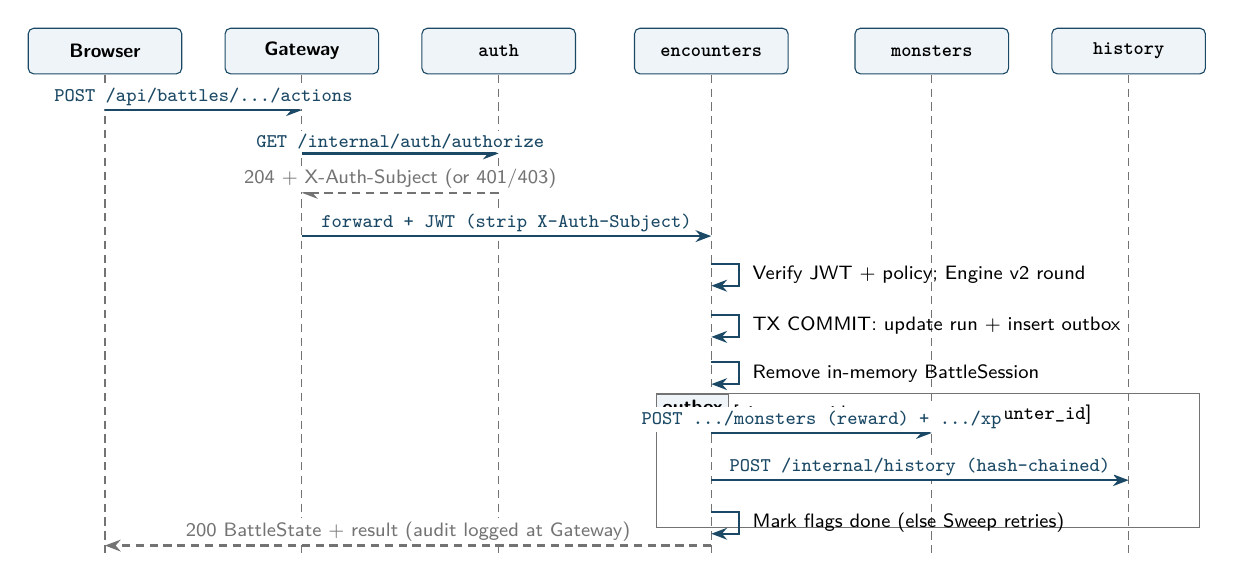
\begin{tikzpicture}[x=1cm, y=1cm]
  % Left diagram: Gateway auth_request + Battle Outbox
  \lifeline{0.0}{Browser}{-6.4}
  \lifeline{2.5}{Gateway}{-6.4}
  \lifeline{5.0}{\code{auth}}{-6.4}
  \lifeline{7.7}{\code{encounters}}{-6.4}
  \lifeline{10.5}{\code{monsters}}{-6.4}
  \lifeline{13.0}{\code{history}}{-6.4}

  \smsg{0.0}{2.5}{-0.75}{POST /api/battles/.../actions}
  \smsg{2.5}{5.0}{-1.30}{GET /internal/auth/authorize}
  \srmsg{5.0}{2.5}{-1.80}{204 + X-Auth-Subject (or 401/403)}
  \smsg{2.5}{7.7}{-2.35}{forward + JWT (strip X-Auth-Subject)}
  \sself{7.7}{-2.70}{Verify JWT + policy; Engine v2 round}
  \sself{7.7}{-3.35}{TX COMMIT: update run + insert outbox}
  \sself{7.7}{-3.95}{Remove in-memory BattleSession}

  \sfrag{7.0}{-4.35}{13.9}{-6.05}{outbox}{victory — idempotent on \code{encounter\_id}}
  \smsg{7.7}{10.5}{-4.85}{POST .../monsters (reward) + .../xp}
  \smsg{7.7}{13.0}{-5.45}{POST /internal/history (hash-chained)}
  \sself{7.7}{-5.85}{Mark flags done (else Sweep retries)}

  \srmsg{7.7}{0.0}{-6.28}{200 BattleState + result (audit logged at Gateway)}
\end{tikzpicture}
\end{adjustbox}
\caption{End-to-end request authorization (\code{INFRA-9}) combined with server-side battle completion and transactional outbox (\code{EN-3}/\code{EN-5}).}
\label{fig:seq-flows}
\end{figure}

% =====================================================================
\section{Resilience, Concurrency \& Performance Engineering}
\label{sec:resilience}
% =====================================================================

Distributed correctness under partial failures and concurrent traffic required five deliberate engineering mechanisms across the backend:

\begin{itemize}
  \item \textbf{Fault Tolerance with 4xx Circuit-Breaker Isolation:} Every internal REST client (\code{PlayersClient}, \code{MonstersClient}, \code{TeamsClient}, \code{EncountersClient}, \code{HistoryClient}, \code{AuthClient}) is guarded by SmallRye Fault Tolerance: \code{@Timeout}, \code{@Retry(maxRetries = 2, delay = 200, abortOn = RemoteClientError.class)}, and \code{@CircuitBreaker(requestVolumeThreshold = 10, failureRatio = 0.5, delay = 5000, skipOn = RemoteClientError.class)} (named \code{RemoteClientException} in \code{players}/\code{teams}). Early testing exposed a subtle microservice anti-pattern: without \code{abortOn}/\code{skipOn}, normal 4xx responses (such as \code{404} or \code{409 TEAM\_INVALID}) counted as circuit-breaker failures and triggered pointless retries, tripping the breaker for healthy traffic. Mapping HTTP 4xx to a dedicated client-error exception and excluding it ensures only genuine infrastructure faults (5xx, timeouts, network errors) retry and open the circuit, returning clean \code{503 DEPENDENCY\_UNAVAILABLE} responses.
  \item \textbf{Transactional Outbox \& Periodic Sweep (\code{EN-5}):} Battle completion persists run progression and a \code{battle\_completions} outbox row in a single PostgreSQL transaction. Remote side effects (\code{reward}, \code{xp}, \code{history}) run post-commit and update individual completion flags. If a downstream service is temporarily down, \code{result.reward.pending = true} is returned honestly to the client, while both lazy recovery on the player's next call and the 1-minute \code{EncounterSweepScheduler} (\code{@Scheduled(every = "\{tamer.sweep.interval:60s\}", concurrentExecution = ConcurrentExecution.SKIP)}) automatically: (1) expire battles idle $>30$ minutes, (2) retry pending outbox rows, and (3) resume runs with \code{reset\_pending = true}. Permanent 4xx remote errors are logged and marked done so they can never deadlock a run reset.
  \item \textbf{Idempotent Internal Writes \& Advisory Locks:} Every mutating \ep{/internal/*} endpoint is idempotent on a natural business key (\code{player\_id} for profile creation, \code{run\_id} for starters/open-run/archive/team-reset/new-run, \code{encounter\_id} for reward/XP/history). In \code{monsters} and \code{teams}, transactional PostgreSQL advisory locks (\code{pg\_advisory\_xact\_lock(hashtext(:key))}) serialize concurrent writes per player/encounter to prevent duplicate inserts or lost updates under retries.
  \item \textbf{Crash-Safe Commit-Before-Eviction Ordering:} In \code{BattleCompletionService.finish()}, the database transaction committing the run update, cleared \code{active\_battle\_*}, and outbox row \emph{always commits before} \code{session.close()} and \code{registry.remove(session)}. If the DB commit fails, the battle remains intact in memory; if the JVM crashes after commit, the outbox guarantees eventual completion of rewards, XP, and history.
  \item \textbf{Fixed 256-Stripe Player Lock Table (\code{BattleRegistry}):} Rather than allocating an unbounded \code{ConcurrentHashMap<UUID,\allowbreak ReentrantLock>} that leaks memory as accounts grow, \code{BattleRegistry} maintains a fixed array of \code{LOCK\_STRIPES = 256} reentrant locks indexed via \code{Math.floorMod(\allowbreak playerId.hashCode(), 256)}. Every state-mutating operation for a player (start, action, abandon, new run, lazy recovery, and background sweep) executes inside \code{withPlayerLock}, guaranteeing strict per-player serialization with $O(1)$ bounded memory.
  \item \textbf{N+1 Query Elimination:} Listing collections and teams initially risked $O(N)$ queries per request. \code{MonsterMapper} batches species and ability lookups using \code{Monster.list("monsterId in ?1", ...)} and \code{Ability.list("abilityId in ?1", ...)}; \code{TeamsService} loads all slots for a player's teams in a single query (\code{TeamSlot.list("teamId in ?1", ...)}); and \code{teams} validates multi-member teams via one batched call to \ep{GET /internal/collections/{pid}/instances?ids=...}.
\end{itemize}

% =====================================================================
\section{Architectural Smells Analysis}
\label{sec:smells}
% =====================================================================

We audited the final architecture against the complete catalog of microservice architectural smells covered in the Advanced Software Engineering lectures. Table~\ref{tab:smells} summarizes each verdict and engineering justification.

\begin{table}[H]
\centering
\caption{Course Architectural Smells audit and mitigation status on the final P2 architecture.}
\label{tab:smells}
\footnotesize
\begin{tabularx}{\linewidth}{@{}L{3.6cm}C{2.15cm}Y@{}}
\toprule
\textbf{Architectural Smell} & \textbf{Verdict} & \textbf{Evidence, Rationale \& Mitigation} \\
\midrule
Endpoint-based Service Interactions & \badgewarn{Present (Allowed)} &
Services address peers via Docker Compose DNS names (\code{https://monsters:8443}) rather than a dynamic service registry. Explicitly permitted by course requirements for static Compose topologies; mitigated by Docker DNS resolver refresh (\code{127.0.0.11 valid=10s}) and env-var injection. \\
\addlinespace
Wobbly Service Interactions & \badgeok{Mitigated} &
Every REST client enforces \code{@Timeout}, \code{@Retry} (with 4xx \code{abortOn}), and \code{@CircuitBreaker} (with 4xx \code{skipOn}), returning \code{503} on outage; critical post-battle and reset workflows use a transactional outbox, idempotent keys, and the 1-min sweep scheduler. \\
\addlinespace
No API Gateway & \badgeok{Absent} &
Nginx acts as the single entry point (\code{127.0.0.1:8443}), providing TLS, routing, CORS, rate limiting, \code{auth\_request} authorization, and JSON request auditing. \\
\addlinespace
Shared Persistence & \badgeok{Absent} &
Strict database-per-service: 6 independent PostgreSQL 17 instances, each isolated on its own \code{<svc>-db-net} internal network with per-service credentials. \\
\addlinespace
Multiple Services in One Container & \badgeok{Absent} &
Strict 1:1 mapping — each microservice, each PostgreSQL DB, the gateway, the frontend, and \code{init-secrets} runs in its own minimal container. \\
\addlinespace
Single-Layer Teams & \badgeok{Absent} &
Work was partitioned vertically by microservice/feature (API, domain logic, Flyway migrations, JUnit tests, Bruno collections), not horizontally by DB/backend/UI layers. \\
\addlinespace
Cyclic Dependency (\code{players} $\leftrightarrow$ \code{encounters}) & \badgewarn{Present (Managed)} &
\code{players} calls \ep{POST /internal/runs} on starter choice; \code{encounters} calls \ep{POST /internal/players/{pid}/new-run} on run reset. \textbf{Why safe:} no Compose startup cycle, disjoint trigger phases (start vs.\ end of run), no recursive call chain, both endpoints idempotent and timeout-protected. \textbf{EN-7 mitigation plan:} if strict acyclicity is required, remove \code{players}$\to$\code{encounters} by having \code{encounters} lazily open a run after querying \ep{GET /internal/players/{pid}}. \\
\addlinespace
Hardcoded Endpoints & \badgeok{Absent} &
Zero hardcoded hostnames/IPs in application code: every peer URL is externalized via \code{TAMER\_<SVC>\_URL} environment variables; frontend uses build-time \code{VITE\_GATEWAY\_URL}. \\
\addlinespace
Inappropriate Service Intimacy & \badgeok{Absent} &
No cross-service DB reads, no shared entity/DTO library (\textbf{A9}), and all internal payloads pass through explicit versioned \ep{/internal/*} OpenAPI contracts. \\
\addlinespace
Microservice Greedy & \badgeok{Evaluated / Justified} &
Six services match the domain's natural security and data-lifecycle boundaries: cryptographic isolation (\code{auth}), append-only auditability (\code{history}), in-memory stateful combat (\code{encounters}), static+owned game data (\code{monsters}), team validation (\code{teams}), and player profile/pool (\code{players}). \\
\bottomrule
\end{tabularx}
\end{table}

% =====================================================================
\section{Frontend Architecture \& Client-Side Assumptions}
\label{sec:frontend}
% =====================================================================

\subsection{Headless Separation, Stack, and Security Controls}

In strict compliance with Requirements §2, the frontend is completely decoupled from the backend:
\begin{itemize}
  \item \textbf{Separate Deployment Stack:} \code{docker-compose.frontend.yml} builds and serves the static bundle from a hardened unprivileged Nginx container on \code{127.0.0.1:8080} (\code{read\_only: true}, \code{mem\_limit: 128m}, \code{pids\_limit: 64}, \code{cap\_drop: ALL}, \code{no-new-privileges:true}). It holds no secrets, joins no backend Docker network, and talks exclusively to \code{https://localhost:8443} from the user's browser via CORS (anchored regex \code{CORS\_ALLOWED\_ORIGINS} allowing ports \code{8080}, \code{5173}, and \code{4173}—never wildcard \code{*}).
  \item \textbf{Minimal Stack, Zero Business Logic:} React 19, TypeScript (DTO types mirror snake\_case API schemas), Vite 8, \code{react-router-dom}, React Context for session state, a typed \code{fetch} client (\code{src/api/client.ts}), and plain CSS pixel-art styling (\code{image-rendering: pixelated}). All dependencies are pinned with \code{package-lock.json} (\code{npm ci}). Pages cover the full loop plus P2 features: \code{/register}, \code{/login}, \code{/starters}, \code{/} (dashboard), \code{/profile} (\code{US-04}), \code{/catalog}, \code{/collection} (with nickname editor, \code{US-13}), \code{/teams}, \code{/encounters}, \code{/battle} (with P2 \code{ability} events), \code{/runs}, and \code{/history} (with live hash-chain verification badge via \ep{GET /api/history/verify}).
  \item \textbf{Single-Flight Refresh Rotation \& Multi-Tab Sync (\code{FE-3}):} Credentials are stored in \code{localStorage} under \code{tamer.session} (\code{\{access\_token, expires\_at, refresh\_token\}}, preserving the refresh credential after access-token expiry so page reload restores the session). Because refresh tokens are single-use rotating credentials (\code{AUTH-7}), submitting the same refresh token twice from parallel API calls or two browser tabs would trigger reuse detection and revoke the session family. \code{FE-3} eliminates this race via a single-flight coordinator and cross-tab storage lock: concurrent callers await one refresh, re-read the updated pair after acquiring the lock, retry the original 401 request at most once, never refresh on \code{403} or auth endpoints, and never auto-retry a refresh after an ambiguous network failure. \textbf{Server Logout:} \code{logout()} serializes against any in-flight refresh, posts \code{refresh\_token} to \ep{POST /api/auth/logout}, invalidates stale responses so a late refresh can never re-authenticate a logged-out user, clears local state in all cases, and surfaces a warning if server revocation failed.
  \item \textbf{XSS \& CSP Hardening:} Zero uses of \code{dangerouslySetInnerHTML} or third-party CDNs; all user strings (\code{display\_name}, team names, nicknames) render strictly as escaped React text. \code{frontend/nginx.conf} sends HTTP headers \code{Content-Security-Policy} (\code{default-src 'self'; script-src 'self'; style-src 'self' 'unsafe-inline'; img-src 'self' data: https://localhost:8443; connect-src 'self' https://localhost:8443; base-uri 'self'; form-action 'self'; object-src 'none'; frame-ancestors 'none'}), \code{Permissions-Policy}, \code{X-Frame-Options: DENY}, \code{X-Content-Type-Options: nosniff}, and \code{Referrer-Policy: no-referrer}, backed by an injected \code{<meta>} CSP in Vite production builds.
\end{itemize}

\subsection{Documented Client-Side Assumptions}

Per \code{docs/plan/09-frontend.md}, the frontend relies on five explicit API contract assumptions:
\begin{enumerate}
  \item The starter pool endpoint (\ep{GET /api/players/me/starters}) returns only species IDs; the client fetches species metadata via \ep{GET /api/monsters?ids=...}.
  \item Sprite URLs returned by the API are relative paths (\ep{/images/monsters/001.png}); the client prefixes \code{VITE\_GATEWAY\_URL}.
  \item The client \textbf{never} computes effective stats, battle damage, XP, team validity, or boss availability; it renders authoritative backend fields (\code{stats}, \code{errors}, \code{result}, \code{boss\_available}).
  \item The team editor invokes \ep{POST /api/teams/validate} on every change for immediate feedback; the backend always re-validates authoritatively on save and battle start.
  \item The battle screen renders \code{last\_round.events} sequentially in server-supplied order; visual animations are strictly cosmetic.
\end{enumerate}

% =====================================================================
\section{Security Architecture, Threat Model \& Verification}
\label{sec:security}
% =====================================================================

\subsection{Requirements §6 Security Compliance Matrix}

\begin{table}[H]
\centering
\caption{Requirements §6 compliance mapping (\code{SEC-1}, \code{docs/plan/11-ci-security.md}).}
\label{tab:sec-compliance}
\footnotesize
\begin{tabularx}{\linewidth}{@{}L{3.5cm}Y L{2.25cm}@{}}
\toprule
\textbf{Requirement (§6)} & \textbf{Implemented Control in Final P2 System} & \textbf{Plan Task} \\
\midrule
Containers in user mode & Non-root \code{USER} in every Dockerfile (\code{10001}, \code{101}, \code{185}, \code{70:70}), \code{read\_only: true}, \code{no-new-privileges:true}, \code{cap\_drop: ALL}, \code{pids\_limit: 256}, \code{mem\_limit}; custom Postgres image without \code{gosu}. & \code{INFRA-2/6} \\
HTTPS/TLS everywhere, per-service certs & Local RSA-4096 CA + per-container RSA-2048 SAN certs via networkless \code{init-secrets}; TLS 1.2/1.3 on gateway, all REST clients (\code{trust-all} forbidden), JDBC \code{sslmode=verify-full}, Postgres \code{pg\_hba.conf} \code{hostssl}. & \code{INFRA-3/4/5} \\
Input sanitisation & Jakarta Bean Validation on every DTO/parameter, Jackson \code{fail-on-unknown-properties=true}, 16 KB Nginx body limit (\code{413}), parameterized Panache/JPA queries. & Conventions, all services \\
Sensitive data encrypted in DB & Usernames encrypted with \textbf{AES-256-GCM} (12-byte random IV) + \textbf{HMAC-SHA256} blind index; passwords bcrypt cost 12; refresh tokens SHA-256 hashed; common-password denylist + login backoff (5 fails / 15 min). & \code{AUTH-7/8} \\
OAuth2 + JWT, secure credentials & OAuth2 \ep{/api/auth/token} (\code{password}, \code{refresh\_token}) \& \ep{/internal/auth/token} (\code{client\_credentials}); RS256 \textbf{300 s} access tokens; rotating opaque refresh tokens (7-day absolute family), reuse family revocation, server logout. & \code{AUTH-3/4/7} \\
AuthN \& operation AuthZ & Defence-in-depth: Nginx \code{auth\_request} (\ep{GET /internal/auth/authorize}, fail-closed \code{503}) + independent service JWT \& \code{AccessPolicyFilter}, both driven by canonical \code{backend/security/access-policy.json} (52 rules). & \code{INFRA-9/10} \\
Access-security regression proof & Real-API positive/401/403 Bruno \code{access/} matrix (component + integration), refresh/logout/replay suites, \code{scripts/check-policy-sync.sh}, CI mutation/negative tests. & \code{TEST-5}, \code{CI-3} \\
Static/dependency scans \& updates & Pinned GitHub Actions SHAs; Semgrep SAST, Trivy \code{fs}/\code{image}/\code{config} in CI; weekly Dependabot across Maven, npm, pip, Actions, and all 10 Dockerfiles. & \code{CI-2}, \code{CI-4} \\
No CRITICAL/HIGH image vulns & Trivy image scan gate; \code{jackson-bom} 2.22.4 override, \code{apk upgrade}, \code{microdnf update}, custom \code{infra/postgres}; 14 unreachable \code{krb5-libs} CVEs tracked with expiry in \code{.trivyignore}. & \code{CI-2} \\
Threat model \& audit evidence & Root \code{THREAT\_MODEL.md} (DFD, 25 STRIDE threats, residual risk ratings); structured JSON audit logs in \code{auth} and \code{gateway} (with verified \code{X-Auth-Subject}), verified 18/18 in CI. & \code{SEC-2/3/4} \\
\bottomrule
\end{tabularx}
\end{table}

\subsection{Tamper-Evident Battle History (\code{HI-2}, \code{US-25})}

To prevent silent tampering or deletion of battle history:
\begin{enumerate}
  \item \textbf{Database Immutability:} Flyway migration \code{V2\_\_append\_only.sql} attaches a PostgreSQL \code{BEFORE UPDATE OR DELETE} trigger on \code{encounter\_records} that unconditionally raises an exception.
  \item \textbf{Per-Player SHA-256 Hash Chain:} Table \code{chain\_heads(player\_id PK, seq, last\_hash)} anchors each player's chain. On \ep{POST /internal/history}, within one transaction, \code{history} acquires a pessimistic lock (\code{SELECT ... FOR UPDATE}) on the player's head row (initializing \code{prev\_hash} to 64 zero hex characters if absent), increments \code{seq}, computes $\text{hash} = \text{SHA-256}(\text{prev\_hash} \parallel \text{canonical\_json}(\text{record}))$ (sorted keys, no whitespace, fixed-precision UTC timestamps), inserts the record, and updates \code{chain\_heads}.
  \item \textbf{Live Verification \& Backups:} \ep{GET /api/history/verify} recomputes the player's entire chain in \code{seq} order and reports \code{\{valid, records, first\_invalid\}}, surfaced directly as an integrity badge in the History UI. Root \code{README.md} documents \code{pg\_dump}/\code{psql} volume backups against data loss.
\end{enumerate}

\subsection{STRIDE Threat Model Summary (\code{SEC-2}) \& Audit Logging (\code{SEC-3}/\code{SEC-4})}

The full threat model resides in \code{THREAT\_MODEL.md} at the repository root. It models \textbf{10 assets} (\code{A1}–\code{A10}), \textbf{7 attack surfaces} (\code{AS1}–\code{AS7}), \textbf{4 trust boundaries} (\code{TB1}–\code{TB4}), and \textbf{25 threats} spanning all six STRIDE categories (\textbf{S}poofing: 3, \textbf{T}ampering: 6, \textbf{R}epudiation: 3, \textbf{I}nformation Disclosure: 6, \textbf{D}enial of Service: 3, \textbf{E}levation of Privilege: 4).

\textbf{Final P2 Threat Posture (27/11/2026):} \textbf{21 Covered} (verified by automated CI tests), \textbf{2 Partial}, and \textbf{2 Gap (accepted)} — \textbf{zero unmitigated high-risk gaps remain}.

\begin{table}[H]
\centering
\caption{Residual risks and accepted decisions from \code{THREAT\_MODEL.md} (§6) after all P2 controls.}
\label{tab:residual-risk}
\footnotesize
\begin{tabularx}{\linewidth}{@{}C{0.7cm}C{1.4cm}C{1.4cm}C{1.3cm}Y@{}}
\toprule
\textbf{\#} & \textbf{Status} & \textbf{Likelihood} & \textbf{Impact} & \textbf{Residual Risk \& Written Decision} \\
\midrule
3  & Partial & low & high   & Compromised container on \code{backend} stealing a caller's client secret (non-callers mount none). \textbf{Accept:} rotate via volume regeneration; use per-caller mTLS in production. \\
7  & Partial & low & high   & TLS 1.2+ verified on every hop + Postgres \code{hostssl}, but no automated rogue-CA integration test. \textbf{Accept:} verified by config checks and TLS 1.1 refusal in CI. \\
8  & Gap     & low & high   & Frontend static bundle served over plain HTTP on \code{127.0.0.1:8080}. \textbf{Accept} for localhost use; place behind HTTPS proxy if exposed externally. \\
13 & Gap     & low & medium & Docker host user can edit/delete stdout \code{json-file} audit logs. \textbf{Accept:} remote append-only WORM log sink out of scope for single-host project. \\
21 & Covered & low & medium & In-memory battle exhaustion bounded by 1 battle/player, 256-stripe lock table, 1-min expiry sweep, and \code{512m} cap. \textbf{Accept} (R19 single-instance design). \\
\bottomrule
\end{tabularx}
\end{table}

\textbf{Entry-Point JSON Audit Logs (\code{SEC-3}, \code{SEC-4}):} Audit lines (\code{ts}, \code{event}, \code{user}, \code{outcome} $\in \{\text{success}, \text{denied}, \text{failure}\}$, \code{request\_id}) are emitted exclusively at the two entry points: \code{auth} (\code{login}, \code{register}, \code{refresh}, \code{refresh\_reuse}, \code{logout}, \code{service\_token} — logging \code{player\_id} on success and the username's HMAC blind index on denial, \textbf{P-27}) and \code{gateway} (\code{log\_format audit}, with \code{escape=json} and \code{user} populated solely from verified \code{X-Auth-Subject}, \textbf{P-28}). \code{scripts/\allowbreak check-audit-log.sh} passed \textbf{18/18} assertions on 27/11/2026, confirming verified \code{.user == \$PLAYER\_ID} correlation and zero leakage of passwords, access tokens, refresh tokens, usernames, or \code{Bearer} headers.

\subsection{CI Security Gates, Trivy Exceptions, and Self-Attack Results (\code{SEC-1})}

GitHub Actions (\code{.github/workflows/ci.yml}, synced with \code{docs/ci/ci.yml}) pins every action to a commit SHA and enforces four security jobs plus weekly Dependabot PRs (\code{.github/dependabot.yml}, \code{CI-4}):
\begin{itemize}
  \item \textbf{Semgrep SAST (\code{sast}):} Rulesets \code{p/java}, \code{p/typescript}, \code{p/react}, \code{p/dockerfile}, \code{p/secrets}, \code{p/owasp-top-ten} — \textbf{0 ERROR findings}; 4 triaged warnings fixed (gateway \code{Host} header override, pinned Action SHAs) or documented false positives.
  \item \textbf{Trivy \code{fs}, \code{image}, \code{config}:} Resolved Maven BOM Jackson CVEs via \code{jackson-bom} 2.22.4, Alpine CVEs via \code{apk upgrade}, Go \code{gosu} CVEs via custom \code{infra/postgres}, and RHEL runtime CVEs via \code{microdnf -y update}. Only one justified, expiring exception remains in \code{.trivyignore}: \textbf{14 HIGH CVEs in \code{krb5-libs} 1.21.1-10.el9\_8.1} inside \code{ubi9/openjdk-21-runtime:1.24}, whose fix is restricted to paid RHEL repos; \code{krb5-libs} is dynamically linked by \code{libcurl}, and all 14 CVEs affect Kerberos KDC/\code{kadmind} daemons not installed or used by any service. Entries expire \textbf{2026-11-30} so CI automatically re-checks upstream UBI packages.
  \item \textbf{Self-Attack Suite (\code{SEC-1}, \code{scripts/security-check.sh}):} Executed against the live hardened stack with real rate limits enabled — \textbf{47/47 checks passed}, covering SQL injection payloads (\code{400}, no stack/SQL leak), JWT attacks (\code{alg:none}, tampered signature, altered payload, expired, missing), cross-player IDOR (\code{404}), \ep{/internal/*} and \ep{/q/*} blocking (\code{404}), forged battle outcome/HP fields (\code{400}), concurrent action/starter races, oversized bodies (\code{413}), XSS text rendering \& HTTP CSP headers, TLS verification (plain HTTP refused, TLS 1.1 rejected, no \code{trust-all}), and brute-force rate limiting (\code{429}).
\end{itemize}

% =====================================================================
\section{Testing, Performance \& Playtest Verification}
\label{sec:testing}
% =====================================================================

\subsection{Automated Test Pyramid Summary}

\begin{table}[H]
\centering
\caption{Complete automated verification results across backend, frontend, API, and security suites (27/11/2026).}
\label{tab:tests}
\footnotesize
\begin{tabularx}{\linewidth}{@{}L{4.0cm}C{1.9cm}C{1.6cm}Y@{}}
\toprule
\textbf{Test Suite / Command} & \textbf{Passed} & \textbf{Failures} & \textbf{Scope \& Per-Component Breakdown} \\
\midrule
Backend JUnit / \code{@QuarkusTest} (\code{mvn clean verify}) & \badgeok{273 / 273} & 0 &
\code{auth} (93), \code{players} (24), \code{monsters} (15), \code{teams} (17), \code{encounters} (96), \code{history} (28). Covers Engine v2 (all 28 abilities), crypto, refresh rotation/reuse, backoff, hash-chain tampering, outbox/sweep, and \code{AccessPolicyTest} in all 6 services. \\
\addlinespace
Frontend Vitest + Lint + Typecheck & \badgeok{16 / 16} & 0 &
Single-flight refresh rotation, multi-tab lock coordination, logout vs.\ stale refresh race (\code{session-refresh.test.ts}); 0 ESLint errors, 0 TypeScript errors, 0 prod \code{npm audit} vulns. \\
\addlinespace
Bruno API Collections (JSON exported) & \badgeok{399 / 399} & 0 &
Component (201 across all 6 services on \code{9001–9006}), Integration (128 via gateway), E2E core loop (36), Access Security Component (17), Access Security Integration (17). \\
\addlinespace
Security \& Policy Scripts & \badgeok{65 / 65+} & 0 &
\code{scripts/security-check.sh} (\textbf{47/47}), \code{scripts/check-audit-log.sh} (\textbf{18/18}), \code{scripts/check-policy-sync.sh} (52 rules verified across all 6 services). \\
\bottomrule
\end{tabularx}
\end{table}

\subsection{Locust Performance Benchmark: Phase 2 vs.\ Phase 1}

Locust (\code{docs/locust/locustfile.py}) drives realistic player sessions exclusively through the HTTPS gateway (\code{https://localhost:8443}): registration, login, starter choice, team creation, catalogue browsing, collection inspection, full turn-by-turn battles, team validation, and history + \ep{/api/history/verify} checks. Table~\ref{tab:locust} compares the final Phase~2 run (\code{docs/locust/results/run\_stats.csv}) against the Phase~1 prototype baseline (\code{docs/locust/README.md}).

\begin{table}[H]
\centering
\caption{Locust load-test results (P2 final from \code{run\_stats.csv} vs.\ P1 baseline). All latencies in ms.}
\label{tab:locust}
\footnotesize
\begin{tabularx}{\linewidth}{@{}L{4.8cm}R{1.15cm}R{1.0cm}R{1.1cm}R{1.1cm}R{1.1cm}R{1.3cm}R{1.2cm}@{}}
\toprule
\textbf{Endpoint (P2 Final Run)} & \textbf{Reqs} & \textbf{Fail} & \textbf{p50} & \textbf{Avg} & \textbf{p95} & \textbf{p99} & \textbf{Req/s} \\
\midrule
\ep{POST /api/battles/current/actions} & 1,383 & 0 & 17   & 40.8  & 150   & 420   & 23.27 \\
\ep{GET /images/monsters/[file]}       & 236   & 0 & 10   & 17.5  & 64    & 120   & 3.97  \\
\ep{GET /api/monsters}                 & 236   & 0 & 25   & 46.8  & 190   & 300   & 3.97  \\
\ep{GET /api/monsters/[id]}            & 236   & 0 & 19   & 37.1  & 140   & 240   & 3.97  \\
\ep{GET /api/encounters}               & 192   & 0 & 25   & 48.5  & 180   & 360   & 3.23  \\
\ep{GET /api/collection}               & 141   & 0 & 27   & 50.3  & 150   & 350   & 2.37  \\
\ep{GET /api/collection/[owned_id]}    & 137   & 0 & 20   & 36.4  & 110   & 170   & 2.30  \\
\ep{GET /api/history}                  & 104   & 0 & 39   & 63.2  & 250   & 320   & 1.75  \\
\ep{GET /api/runs/current}             & 101   & 0 & 20   & 43.8  & 140   & 410   & 1.70  \\
\ep{POST /api/battles} (start)         & 91    & 0 & 91   & 134.4 & 480   & 920   & 1.53  \\
\ep{GET /api/history/[encounter_id]}   & 79    & 0 & 20   & 36.1  & 120   & 360   & 1.33  \\
\ep{POST /api/teams/validate}          & 55    & 0 & 70   & 83.4  & 200   & 430   & 0.93  \\
\ep{POST /api/players/me/starters}     & 32    & 0 & 230  & 229.1 & 370   & 400   & 0.54  \\
\ep{POST /api/teams} (create)          & 32    & 0 & 200  & 213.9 & 380   & 390   & 0.54  \\
\ep{GET /api/history/verify} (P2 new)  & 30    & 0 & 27   & 55.0  & 180   & 530   & 0.50  \\
\ep{POST /api/auth/register} (bcrypt)  & 30    & 0 & 2,300 & 2,243.5 & 3,800 & 4,200 & 0.50  \\
\ep{POST /api/auth/token} (bcrypt)     & 30    & 0 & 2,300 & 2,198.3 & 3,600 & 3,800 & 0.50  \\
\emph{Other reads} (\code{abilities}, \code{elements}, \code{starters}, \code{PUT team}) & 189 & 0 & 14–77 & 27–109 & 120–310 & 200–370 & 3.18 \\
\midrule
\textbf{P2 Aggregated (27/11/2026)}    & \textbf{3,334} & \textbf{0 (0.00\%)} & \textbf{20} & \textbf{87.1} & \textbf{230} & \textbf{2,300} & \textbf{56.09} \\
\textbf{P1 Baseline (09/11/2026)}      & \textbf{11,667} & \textbf{23 (0.20\%)} & \textbf{61} & — & \textbf{1,100} & \textbf{4,100} & \textbf{$\approx$65.0} \\
\bottomrule
\end{tabularx}
\end{table}

\textbf{Performance Analysis:} Despite Phase~2 adding substantial security overhead—gateway \code{auth\_request} subrequests on every protected call, AES-256-GCM encryption + HMAC indexing, rotating refresh tokens, and row-locked SHA-256 history chaining—\textbf{P2 achieved 0.00\% failures} (eliminating all 23 P1 \code{503} circuit-breaker trips on battle start and team validation) while cutting overall median latency from \textbf{61 ms $\to$ 20 ms} ($-67\%$) and \code{p95} from \textbf{1,100 ms $\to$ 230 ms} ($-79\%$). Battle actions—the dominant gameplay hot path—resolved in \textbf{17 ms median} (\code{p95} 150 ms) thanks to the in-memory engine and fixed 256-stripe lock table. Only \ep{/register} and \ep{/token} exhibit $\sim$2.3 s latency during burst startup, which is the deliberate bcrypt cost-12 defence against offline/online brute forcing and runs once per session.

\subsection{Full Interactive Browser Playtest \& Backlog Traceability}

\textbf{Interactive E2E Playtest:} Beyond automated suites, we executed a complete live browser playthrough against the containerized frontend (\code{http://localhost:8080}) and gateway (\code{https://localhost:8443}), progressing from fresh account registration and profile customization through all 8 stages, earning wild and boss monsters, tuning teams, observing P2 abilities (\code{heal}, \code{reflect}, \code{stun}, \code{revive}, \code{invert\_advantage}) live in the round log, and defeating Stage~8 Final Boss \textbf{Omnivoid} on \textbf{Turn 23} (run status \code{won}), concluding with \textbf{30 verified hash-chained history records} confirmed green by both \ep{GET /api/history/verify} and the UI integrity badge.

\begin{table}[H]
\centering
\caption{User story \& acceptance-criteria traceability (\code{docs/backlog/acceptance\_criteria.md} \& \code{.xlsx}).}
\label{tab:backlog}
\footnotesize
\begin{tabularx}{\linewidth}{@{}L{2.3cm}C{1.1cm}L{3.9cm}Y@{}}
\toprule
\textbf{Priority / Count} & \textbf{Phase} & \textbf{Story IDs} & \textbf{Functional Coverage \& Primary Verification} \\
\midrule
\textbf{Red (18)} Mandatory & P1 &
\code{US-01}–\code{03}, \code{US-06}, \code{US-09}–\code{12}, \code{US-14}–\code{20}, \code{US-23}, \code{US-24}, \code{US-28} &
Full registration, OAuth2 login, progress resume, starter pool, catalogue/details/sprites, collection \& rewards, team CRUD/validation, 8-stage encounters, server-side battle resolution \& results, history list/detail, web UI. Verified by JUnit, Bruno (component/integration/e2e), and full browser playtest. \\
\addlinespace
\textbf{Yellow (2)} Security/Integrity & P1+P2 &
\code{US-05} (account protection), \code{US-25} (anti-tampering) &
404 anti-IDOR, TLS everywhere, 300 s JWT + refresh rotation/logout, AES-GCM/HMAC username encryption, backoff, gateway \code{auth\_request}, append-only trigger + SHA-256 hash chain + \ep{/api/history/verify}. Verified by JUnit, Bruno \code{access/}, \code{SEC-1} (47/47), \code{check-audit-log.sh} (18/18). \\
\addlinespace
\textbf{Green (5)} Optional & P1+P2 &
\code{US-04} (profile edit), \code{US-07} (pick starters), \code{US-13} (nicknames), \code{US-21} (flee/abandon), \code{US-22} (battle actions) &
\ep{PATCH /api/players/me} + \code{/profile} page; 3-of-10 starter selection; \ep{PATCH /api/collection/{id}} custom nicknames; battle \code{flee} + run \code{abandon}; explicit \code{attack}/\code{switch}/\code{flee} controls. Documented in OpenAPI, \code{acceptance\_criteria.md}, and UI. \\
\bottomrule
\end{tabularx}
\end{table}

% =====================================================================
\section{Known Limitations \& Oral-Exam Quick Reference}
\label{sec:limitations-oral}
% =====================================================================

\subsection{Known Limitations and Production Evolution Paths}

\begin{enumerate}
  \item \textbf{In-Memory Active Battles / Single \code{encounters} Instance (R19):} Active battles live in memory inside \code{BattleRegistry} (\code{ConcurrentHashMap}). A restart loses active round state (gracefully closed as \code{interrupted} on recovery without losing the run or collection), and \code{encounters} cannot horizontally scale as-is. \emph{Evolution:} externalize active battle snapshots to Redis with optimistic versioning or sticky routing.
  \item \textbf{Local CA, Plain-HTTP Localhost Frontend, and Stdout Audit Logs (Threats \#8, \#13):} Appropriate for a single-host academic deployment, but production would replace the self-signed CA with ACME/enterprise PKI, serve the frontend over HTTPS, and ship JSON audit streams to a remote WORM log collector.
  \item \textbf{Expiring UBI9 \code{krb5-libs} Trivy Exception:} 14 unreachable Kerberos KDC/\code{kadmind} CVEs in \code{ubi9/openjdk-21-runtime:1.24} are ignored in \code{.trivyignore} until \code{2026-11-30}, when CI re-evaluates upstream UBI patches.
  \item \textbf{Stateless 300 s Access-Token Revocation Window (\code{AUTH-7}):} Logout and reuse detection immediately block all future refreshes, while already-minted access JWTs expire naturally within at most 300 s (+ clock skew). Eliminating that window would require a distributed revocation cache, trading away stateless local verification.
  \item \textbf{Managed \code{players} $\leftrightarrow$ \code{encounters} Call Cycle:} Safe today (disjoint lifecycle, no startup dependency), with a documented \code{EN-7} lazy-run creation refactor to remove the cycle entirely if desired.
\end{enumerate}

\subsection{Oral-Exam Quick Reference (Key Engineering Talking Points)}

\begin{table}[H]
\centering
\caption{High-yield architecture, resilience, and security rationale for individual oral defense.}
\label{tab:oral}
\footnotesize
\begin{tabularx}{\linewidth}{@{}L{4.2cm}Y@{}}
\toprule
\textbf{Likely Exam Question} & \textbf{Crisp, Evidence-Backed Answer} \\
\midrule
Why 6 services and synchronous REST instead of a monolith or Kafka? &
Six bounded contexts align with security/data lifecycles (isolating crypto keys in \code{auth} and append-only records in \code{history}) and vertical 4-person ownership. Sync REST keeps one paradigm; eventual consistency where needed (post-battle rewards/XP/history and run reset) is solved cleanly with a transactional outbox + idempotent keys + 1-min sweep scheduler without operating a message broker. \\
\addlinespace
How did you fix circuit breakers tripping under normal traffic? &
Internal REST clients map 4xx responses to \code{RemoteClientError}/\code{RemoteClientException} and pass it to \code{@Retry(abortOn = ...)} and \code{@CircuitBreaker(skipOn = ...)}. Client errors (\code{404}/\code{409}) pass straight through without retrying or counting toward the failure ratio, while 5xx/timeouts still trip the breaker and fail fast with \code{503}. \\
\addlinespace
How do gateway and services avoid authorization policy drift? &
One canonical \code{backend/security/access-policy.json} (52 rules) is packaged into every service and checked in CI (\code{check-policy-sync.sh}). Nginx delegates every protected route via internal HTTPS \code{auth\_request} to \code{auth}'s \ep{/internal/auth/authorize} (fail-closed \code{503}), and each service independently re-verifies the RS256 JWT and the exact same policy (\code{AccessPolicyFilter}). \\
\addlinespace
Why return 404 instead of 403 for another player's resource? &
Decision \textbf{P-11}: returning \code{403} confirms a foreign UUID exists (object-enumeration oracle). Scoping every repository query by \code{player\_id} from the JWT \code{sub} claim returns \code{404} identically for missing and foreign IDs. \\
\addlinespace
How do you query encrypted usernames at login? &
\textbf{AUTH-8}: AES-256-GCM uses a random 12-byte IV, so ciphertexts are non-deterministic and unindexable. We pair it with a keyed \textbf{HMAC-SHA256 blind index} over the normalized lowercase username for $O(1)$ unique lookup and safe denied-login audit correlation (\textbf{P-27}) without ever storing or logging plaintext usernames. \\
\addlinespace
How does the history hash chain stay consistent under concurrency? &
\textbf{HI-2}: \ep{POST /internal/history} executes inside one transaction that acquires \code{SELECT ... FOR UPDATE} on the player's \code{chain\_heads} row before assigning \code{seq} and hashing \code{prev\_hash || canonical\_json}. Concurrent inserts for the same player serialize cleanly; a DB trigger blocks \code{UPDATE}/\code{DELETE}. \\
\addlinespace
How does the frontend avoid refresh-token replay revocations? &
\textbf{FE-3}: Rotating refresh tokens are single-use; two parallel 401 responses or two open tabs sending the same token would trigger reuse family revocation. The client uses a single-flight coordinator + cross-tab lock, re-reads storage after acquiring the lock, and serializes logout so stale refresh responses cannot restore a logged-out session. \\
\addlinespace
Why did P2 Locust perform better than P1 despite heavier security? &
P2 eliminated all 23 P1 \code{503} errors (0.00\% failures across 3,334 reqs) and reduced median latency from 61 ms to 20 ms (\code{p95} 1,100 ms $\to$ 230 ms) via 4xx circuit-breaker exclusion, batched N+1 queries in \code{monsters}/\code{teams}, and fixed 256-stripe locking in \code{encounters}. \\
\bottomrule
\end{tabularx}
\end{table}

\end{document}
